\documentclass[journal,twocolumn,10pt]{IEEEtran}

\usepackage{amsmath,amssymb,amsthm}
\usepackage{booktabs}
\usepackage{graphicx}
\usepackage{cite}
\usepackage{url}
\usepackage{xcolor}
\usepackage{tikz}
\usetikzlibrary{positioning,arrows.meta,fit,backgrounds}
\usepackage[hidelinks]{hyperref}

\graphicspath{{figures/}}
\input{generated_tables/autogen_metrics.tex}
\input{generated_tables/gen_metrics.tex}
\input{generated_tables/val_metrics.tex}
\newtheorem{proposition}{Proposition}

\begin{document}

\title{When Does Split Computing Pay Off for UAV Object Detection?\\A Measured and Trace-Driven Study with YOLOv8}

\author{Utkarsh~Sengar%
\thanks{U.~Sengar is with the Department of Computer Science \& Engineering, Indian Institute of Technology Dharwad, Karnataka 580011, India (e-mail: cs23bt026@iitdh.ac.in). This work was carried out as a B.Tech.\ project. Code, data-preparation scripts, and every result file are released with the paper.}}

\markboth{B.Tech Project Report, Department of CSE, IIT Dharwad}{Sengar: When Does Split Computing Pay Off for UAV Object Detection?}

\maketitle

\begin{abstract}
Split computing runs a detector's first layers onboard and sends the intermediate activations to a server, a common proposal for UAVs that cannot run detection fast enough onboard. For an off-the-shelf YOLOv8s, we ask whether splitting beats onboard inference or image offloading. Our toolkit, AEGIS-UAV, splits the detector exactly at any of its 22 layer boundaries and streams the quantized crossing tensors in an authenticated wire format. INT8 quantization changes mAP@[.5:.95] on COCO val2017 by at most \MaxAbsDeltaINT{} points at any cut. The payload is the obstacle: the smallest split payload (\MinSplitKiB{}~KiB at \MinSplitCut{}, with lossless zstd) is \RatioMinSplitOverJPEGQNinetyFive$\times$ a Q95 JPEG frame that loses only \JPEGDeltaQNinetyFive{} points. In trace-driven simulation, JPEG offload is the best fixed strategy in all \NumCells{} channel and onboard-speed settings, while splitting beats onboard inference in \SplitBeatsOnboardCells{}. An adaptive policy matches or exceeds fixed JPEG in all \NumCells{} settings and falls below it in \GenAdaptiveBelowJpegN{} of \GenAdaptiveScenariosN{} random systems, by at most \GenAdaptiveVsJpegWorstPct\,\%. Relaying between UAVs rarely helps. Across \GenNModels{} detectors from \GenNFamilies{} YOLO families, five input sizes, and aerial imagery, the smallest split payload is \GenRatioMin--\GenRatioMax$\times$ a Q90 JPEG frame, and fewer bits lose accuracy faster than JPEG at equal size. A closed-form model, checked on \GenNScenarios{} + \GenNSwarmScenarios{} random systems, shows why: a split can beat an image needing fewer bits and less onboard work only by its accuracy ratio (at most \GenMaxSplitGainPct\,\% observed). Post-hoc quantized splitting is accurate but not bandwidth-competitive; we release the toolkit for evaluating learned bottlenecks.
\end{abstract}

\begin{IEEEkeywords}
Split computing, UAV, object detection, YOLOv8, feature quantization, computation offloading, trace-driven evaluation.
\end{IEEEkeywords}

\section{Introduction}
\IEEEPARstart{U}{AVs} used for inspection, search and rescue, or surveillance need object detection at video rate, yet the embedded computers they can carry are power- and weight-limited~\cite{mozaffari2019tutorial,zeng2016wireless}. Cellular connectivity makes offloading attractive~\cite{zeng2019cellular}, and \emph{split computing}---running the head of a network onboard and the tail on a server---has been proposed as a middle ground between onboard inference and sending images~\cite{kang2017neurosurgeon,matsubara2022survey}.

Whether splitting helps depends on a comparison that is easy to get wrong: intermediate activations of a detector are large, often larger than the input image~\cite{matsubara2022survey}, while standard image codecs are extremely efficient. A fair evaluation must (i) measure accuracy on held-out data with the actual quantization applied at the cut, (ii) compare against a properly compressed image, and (iii) model a finite uplink, finite onboard compute, and a deadline in the same framework. This paper does all three for YOLOv8s~\cite{redmon2016you,jocher2023yolo}.

\textbf{Contributions.}
\begin{itemize}
\item \emph{Toolkit.} AEGIS-UAV splits YOLOv8s at any layer boundary by computing the set of activations that cross the cut; edge-then-cloud outputs are bit-identical to the unsplit model at all 22 cuts. It includes an authenticated, fail-closed wire format, a server that serves every cut from one copy of the weights, and a C++/CUDA INT8 quantizer that is bit-identical to the Python reference (Section~\ref{sec:toolkit}).
\item \emph{Accuracy.} On COCO val2017 we quantize exactly the crossing tensors per image and report paired-bootstrap confidence intervals. INT8 costs at most \MaxAbsDeltaINT{} mAP@[.5:.95] points at every cut; percentile clipping, often assumed to help, measurably hurts (Section~\ref{sec:accuracy}).
\item \emph{Rate.} Every YOLOv8s cut needs at least \RatioMinSplitOverJPEGQNinetyFive$\times$ the bytes of a Q95 JPEG frame, even after lossless entropy coding, for an accuracy difference of about 0.2 points (Section~\ref{sec:rate}).
\item \emph{System evaluation.} One explicit model (finite link, sequential onboard processor, newest-frame buffering, deadline, cell sharing) evaluates onboard, split, JPEG, and adaptive strategies over synthetic channel traces and a sweep of onboard speeds. It covers one UAV and swarms with relaying, and it includes an uncertainty-aware adaptive policy (Sections~\ref{sec:model}--\ref{sec:system}).
\item \emph{Generalization.} We derive closed-form conditions, in terms of every system parameter, for when image offload dominates splitting and when splitting beats onboard inference. We verify them on \GenNScenarios{} + \GenNSwarmScenarios{} randomly drawn systems and support them with measurements on \GenNModels{} detectors, input sizes from \GenResSizeSmall{} to \GenResSizeLarge~px, 2--8-bit wire formats, and aerial imagery (Section~\ref{sec:generalization}).
\end{itemize}
The central finding is a negative result. For an unmodified detector, post-hoc quantized splitting is essentially lossless and often better than onboard inference. It did not, however, beat JPEG offload in any of the \NumCells{} system-level settings, and in randomly drawn systems it won by at most \GenMaxSplitGainPct\,\%. This points to learned bottleneck compression~\cite{matsubara2023sc2,shao2020bottlenetpp} rather than post-hoc quantization of existing layers.

\section{Background and Related Work}
\textbf{Split computing.} Neurosurgeon~\cite{kang2017neurosurgeon} chose the partition point from per-layer latency and energy profiles. Later work extended partitioning to DAG-structured networks (DADS~\cite{hu2019dads}), compressed the transferred features (JALAD~\cite{li2018jalad}), and selected the split according to the available bandwidth (Edgent~\cite{li2020edgent}); SPINN~\cite{laskaridis2020spinn} combined splitting with early exits. Matsubara \emph{et al.}~\cite{matsubara2022survey} survey the area and observe that the early layers of vision models often produce more data than the input, which limits naive splitting.

\textbf{Feature compression.} Choi and Baji\'{c}~\cite{choi2018deep} compressed detector features with standard codecs. BottleNet~\cite{eshratifar2019bottlenet} and BottleNet++~\cite{shao2020bottlenetpp} learn a bottleneck jointly with the task, and supervised compression~\cite{matsubara2022supervised} and the SC2 benchmark~\cite{matsubara2023sc2} show that learned encoders can beat input-image coding. We deliberately study the training-free case instead: an existing detector with post-hoc quantization~\cite{jacob2018quantization,krishnamoorthi2018quantizing}, which a practitioner can deploy without retraining.

\textbf{UAV links and computation.} Cellular-connected UAVs see channels dominated by line of sight but still variable~\cite{zeng2019cellular,3gpp36777}, and UAV offloading studies usually model the network analytically~\cite{mozaffari2019tutorial}. We instead use trace-driven simulation, which couples the link to onboard processing and a deadline.

\section{The AEGIS-UAV Toolkit}\label{sec:toolkit}

\begin{figure*}[t]
\centering
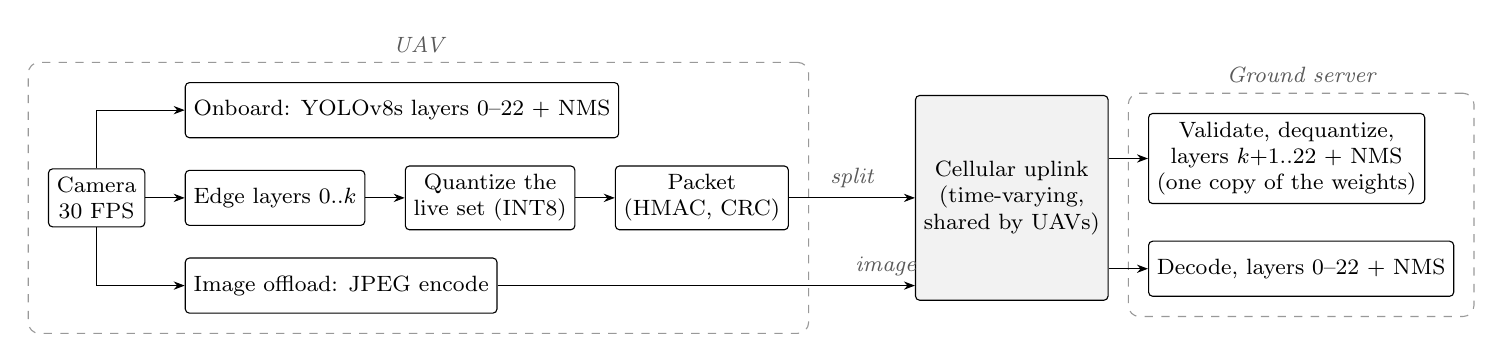
\begin{tikzpicture}[
  font=\footnotesize, >={Stealth[length=4pt]}, node distance=4mm and 5mm,
  blk/.style={draw, rounded corners=1.5pt, minimum height=7mm, inner sep=3pt, align=center, fill=white},
  lbl/.style={font=\footnotesize\itshape, text=black!65}]
  \node[blk] (cam) {Camera\\30 FPS};
  \node[blk, right=of cam] (edge) {Edge layers $0..k$};
  \node[blk, right=of edge] (q) {Quantize the\\live set (INT8)};
  \node[blk, right=of q] (pkt) {Packet\\(HMAC, CRC)};
  \node[blk, above=of edge.north west, anchor=south west, minimum width=38mm] (full) {Onboard: YOLOv8s layers 0--22 + NMS};
  \node[blk, below=of edge.south west, anchor=north west] (jpg) {Image offload: JPEG encode};
  \node[blk, right=16mm of pkt, minimum height=26mm, fill=black!5] (link) {Cellular uplink\\(time-varying,\\shared by UAVs)};
  \node[blk, right=of link, yshift=5mm] (cloud) {Validate, dequantize,\\layers $k{+}1..22$ + NMS\\(one copy of the weights)};
  \node[blk, right=of link, yshift=-9mm] (dec) {Decode, layers 0--22 + NMS};
  \draw[->] (cam) |- (full);
  \draw[->] (cam) -- (edge);
  \draw[->] (cam) |- (jpg);
  \draw[->] (edge) -- (q);
  \draw[->] (q) -- (pkt);
  \draw[->] (pkt) -- node[above, lbl] {split} (link.west |- pkt);
  \draw[->] (jpg) -- node[above, lbl, pos=0.93] {image} (link.west |- jpg);
  \draw[->] (link.east |- cloud) -- (cloud);
  \draw[->] (link.east |- dec) -- (dec);
  \begin{scope}[on background layer]
    \node[draw=black!40, dashed, rounded corners, fit=(cam)(full)(pkt)(jpg), inner sep=2.5mm, label={[lbl]above:UAV}] {};
    \node[draw=black!40, dashed, rounded corners, fit=(cloud)(dec), inner sep=2.5mm, label={[lbl]above:Ground server}] {};
  \end{scope}
\end{tikzpicture}
\caption{The three strategies compared. The toolkit implements the split path end to end (edge and cloud processes, wire format, dispatcher); the simulator of Section~\ref{sec:model} models all three paths with measured payload sizes and processing times.}
\label{fig:arch}
\end{figure*}
\subsection{Exact splitting of a DAG-structured detector}
Fig.~\ref{fig:arch} shows the three ways a frame can be processed. YOLOv8s (\TotalParamsM{}M parameters, \TotalGFLOPs{} GFLOPs at 640$\times$640) has 23 modules with skip connections from its backbone to its neck. Cutting after module $k$ therefore requires sending every activation produced at or before $k$ that a module after $k$ consumes. We compute this \emph{live set} from the module graph; for example it is $\{4\}$ for $k{=}4$, $\{4,6,9\}$ for $k{=}9$, and $\{9,15,18\}$ for $k{=}18$ (Table~\ref{tab:splits}). The edge submodel returns the live set; the cloud submodel accepts exactly that set and rejects anything else. Because both halves execute the same kernels on the same tensors, edge-then-cloud output is bit-identical to the unsplit model; our tests check this at all 22 cuts.

\subsection{Quantization at the boundary}
Each crossing tensor $X$ is quantized independently per frame. Per-tensor symmetric INT8 computes the scale $S=\max|X|/127$ and rounds it to float32, so the value carried on the wire is exactly the one used ($S=1$ if $\max|X|<10^{-6}$). The codes are $q=\mathrm{clamp}(\mathrm{round}(X/S),-128,127)$ with round-half-to-even, and per-channel INT8 uses one such scale $S_c$ per channel. We also implement affine UINT8, FP16, and lossless zstd~\cite{rfc8878zstd} coding of the INT8/UINT8 bytes.
\begin{proposition}\label{prop:int8}
For symmetric INT8, $\|X-\hat X\|_\infty \le S/2$ in exact arithmetic, where $\hat X = qS$ (per channel, the error in channel $c$ is at most $S_c/2$).
\end{proposition}
\begin{proof}
Rounding $\max|X|/127$ to float32 changes it by a relative error below $2^{-23}$, so $|X_i/S|\le127/(1-2^{-23})<127.5$. Hence $\mathrm{round}(X_i/S)\in[-127,127]$, the clamp is inactive, and $|X_i/S-\mathrm{round}(X_i/S)|\le\frac12$; multiply by $S$. If $\max|X|<10^{-6}$, then $q=0$ and the error is below $10^{-6}<S/2$. The per-channel case is the same argument for each channel.
\end{proof}
Evaluating $\hat X$ in float32 adds at most about one unit in the last place of $\max|X|$, and on real $k_4$ activations the largest observed ratio $\max|X-\hat X|/(S/2)$ is \BoundRatioMax{}. The bound is elementary. We state it because it lets the receiver know the worst-case feature error from the header alone.

\subsection{Wire format and server}
A packet carries a 16-byte header (version, frame id, capture timestamp, cut, tensor count, flags), a 16-byte descriptor per tensor (layer, dtype, $C,H,W$, scale, payload length), the payloads, an optional HMAC-SHA256 tag, and a CRC32. Parsing is fail-closed. The parser rejects unknown dtypes, dimension mismatches, trailing bytes, inconsistent flags, over-sized decompression, and missing or wrong authentication tags, and the server counts and drops such packets instead of crashing. Transport uses ZeroMQ~\cite{hintjens2013zeromq} with bounded queues and message sizes. The server holds one copy of the weights and builds a lightweight view for each requested cut, validating cut codes from the network before it uses them.

\subsection{CUDA quantizer}
A two-kernel CUDA implementation (a max-abs reduction, then quantization) runs on PyTorch's current stream and reproduces the Python quantizer bit for bit, including round-half-to-even and the float32 scale. The test suite builds it and checks equality on the GPU. One subtlety matters here: PyTorch implements division of a CUDA tensor by a Python scalar as multiplication by a reciprocal, so the reference divides by a float32 tensor to make results device-independent.

\section{Measurement and System Model}\label{sec:model}
\subsection{Accuracy protocol}
All accuracy numbers use the \NumValImages{} COCO val2017 images~\cite{lin2014microsoft}, none of which were used to train YOLOv8s, with the standard Ultralytics protocol (letterboxing, confidence 0.001, IoU 0.7, 101-point interpolation). For each configuration, forward hooks quantize and dequantize exactly the live tensors at the point where the cloud consumes them, so edge-side layers keep full-precision inputs. A test verifies that this gives the same result as running the real edge, quantizer, and cloud. Validation uses batch size 1, so every image gets its own scales. Differences from the FP32 baseline (mAP@[.5:.95] = \BaselineMAP, mAP@.5 = \BaselineMAPfifty) are reported with 95\% confidence intervals from a paired percentile bootstrap over images~\cite{efron1993bootstrap} (\NBootAccuracy{} resamples; \NBootCodec{} for the codec baselines). FP32 splits are exact by construction, and we confirm this end to end for $k_4$.

\subsection{Rate and timing}
We measure wire sizes by serializing real activations of \TimingImages{} letterboxed val2017 frames. The codec baselines encode the same frames with JPEG~\cite{wallace1992jpeg} and WebP (OpenCV) and with H.264~\cite{wiegand2003h264} (libx264, intra-only single frames, ``ultrafast/zerolatency''). Single-frame H.264 is a pessimistic stand-in for video coding with inter prediction. Codec accuracy is measured by running detection on the decoded frames. Host timings are measured per stage on an \HostGPU{}, after warm-up and with CUDA synchronisation (Table~\ref{tab:timing}). Their NMS uses deployment settings (confidence 0.25, IoU 0.45), whereas accuracy uses the validation settings above.

\subsection{Onboard hardware as a parameter}\label{sec:model-hw}
We do not have measurements on a UAV computer, so onboard speed is a parameter rather than a claim. Let $t_{full}$ be the onboard latency of the whole model and $t^{host}_{full}$ the same latency measured on the host. A configuration $c$ is onboard inference, a split at cut $k$, or an image codec. Let $\phi_c$ be the fraction of the model's FLOPs it executes onboard ($\phi=1$ onboard, $\phi_k$ from Table~\ref{tab:splits}, $\phi=0$ for a codec), and $\rho_c$ the host-measured time of its other onboard work (quantization and serialization, or image encoding) divided by $t^{host}_{full}$ ($\rho=0$ onboard). The DNN part scales with its FLOPs and the other work by the same factor $t_{full}/t^{host}_{full}$, so the onboard time is
\begin{equation*}
e_c = t_{full}\,(\phi_c+\rho_c).
\end{equation*}
We report results for $t_{full}\in\{40,90,180,360\}$~ms, spanning a well-optimised embedded accelerator to an unoptimised one. Server times $s_c$ are the measured host times (deserialization, dequantization, the cloud layers, and NMS; or decoding and the whole model). The power figures in Table~\ref{tab:params} are assumptions, not measurements. Energy is the busy-time-weighted increment above idle, so the average perception power is
\begin{align*}
P_{\mathrm{perc}} = P_{\mathrm{idle}}+P_{rx} &+ (P_{\mathrm{busy}}-P_{\mathrm{idle}})\,u_{\mathrm{cmp}}\\
&+ (P_{tx}-P_{rx})\,u_{tx}+P_{a2a}\,u_{a2a},
\end{align*}
where $u_{\mathrm{cmp}},u_{tx},u_{a2a}\in[0,1]$ are the fractions of time the compute module, the modem, and the air-to-air radio are busy.

\subsection{Channel traces}
Traces are \emph{synthetic}, and we label them as such. In dB, the SINR $\gamma$ of each 10~ms slot is the sum of a mean, log-normal shadowing, and Rician block fading. The shadowing has Gudmundson spatial correlation~\cite{gudmundson1991correlation}: it is an AR(1) process in dB whose correlation between positions $\Delta x$ apart is $e^{-\Delta x/d_{corr}}$. The fading follows a Clarke Doppler spectrum~\cite{clarke1968statistical} at 3.5~GHz; we simulate it at 1~kHz and average it over each slot. Throughput is $W\cdot\mathrm{SE}(\gamma)$ for an uplink bandwidth $W$, with the attenuated and truncated Shannon bound of 3GPP TR 36.942~\cite{3gpp36942}: $\mathrm{SE}(\gamma)=\min(\alpha\log_2(1+\gamma),\mathrm{SE}_{max})$ for $\gamma\ge\gamma_{min}$ and 0 below ($\alpha=\ShannonAlpha$, $\mathrm{SE}_{max}=\ShannonSEMax$~bit/s/Hz, $\gamma_{min}=\ShannonSINRMin$~dB). Each slot also carries a one-way delay and a residual loss. The delay is a profile-specific base of 10--20~ms plus $10(1-\mathrm{SE}/\mathrm{SE}_{max})$~ms plus exponential jitter with mean 2~ms, so it grows as the link degrades. The residual post-HARQ loss of $0.1\,e^{-(\gamma-\gamma_{min})/3}$\,\% ($\gamma$ in dB) is at most 0.1\,\% while the link is up and 100\,\% in outage. Four profiles are used: \emph{good} (mean \TraceGoodMeanMbps~Mbps), \emph{moderate} (\TraceModerateMeanMbps~Mbps, 5th percentile \TraceModeratePFiveMbps), \emph{blackout} (\TraceBlackoutMeanMbps~Mbps with two 3~s deep fades, \TraceBlackoutOutagePct\% outage), and \emph{fast fading} (\TraceFadingMeanMbps~Mbps, 5th percentile \TraceFadingPFiveMbps). Each simulation seed, and each UAV in a swarm, draws an independent realisation with independently timed blackouts; only the reference trace released with the code uses fixed blackout times. Measured traces in the same format can be substituted.

\subsection{Simulator}
The simulator advances in 10~ms slots and treats each UAV as a pipeline. A camera at $F=30$~FPS captures frames. A sequential onboard processor handles one frame at a time and skips frames that arrive while it is busy, and processed frames wait in a newest-frame-wins uplink buffer. The link's goodput is the trace bandwidth times one minus the residual loss. In a shared cell this goodput is water-filled across the UAVs that are transmitting: each receives its own goodput or an equal share of the capacity left over, whichever is smaller. Every frame faces a deadline $D$, and a transfer is dropped once its frame is older than the 300~ms deadline. A frame is \emph{on time} if its result is available within $D$ of capture. An offloaded frame's result becomes available at the server, after the onboard time, queueing, transmission, the trace's one-way delay, and the server time. Under onboard inference the result is available onboard, after $t_{full}$. Our main metric is on-time frames per second per UAV. Results are means over \NumSeeds{} seeds with 95\% $t$-intervals.

Relaying is optional. When a UAV's goodput estimate falls below \RelayThresholdMbps~Mbit/s, it sends each ready frame over an 802.11ax air-to-air link to the neighbour with the highest estimate above \RelayNeighbourMinMbps~Mbit/s, where the frame competes for that neighbour's uplink. The air-to-air link uses log-distance path loss at 5.8~GHz with static log-normal shadowing per UAV pair ($\sigma_{a2a}=\AtwoAShadowDb$~dB, the same in both directions). Link adaptation picks the MCS $j$ (20~MHz, one stream) that maximises $r_j(1-\mathrm{PER}_j)$. Here $\mathrm{PER}_j$ is \AtwoAPerThreshold\,\% at the MCS's SNR threshold (the 802.11 receiver-sensitivity criterion), changes by one decade per \AtwoAPerSlope~dB around it, and is capped at 1; a MAC efficiency of \AtwoAMacEff{} accounts for protocol overhead. At the \AtwoASpacingM~m formation spacing this gives \AtwoASpacingMbps~Mbit/s without shadowing, and goodput reaches zero at about \AtwoARangeM~m.

\subsection{Validation}\label{sec:validation}
The simulator abstracts the network, so we checked it against two independent packet-level simulators, ns-3.48~\cite{riley2010ns3} and OMNeT++~6.3~\cite{varga2008omnetpp} with INET~4.5~\cite{meszaros2019inet} and Simu5G~1.6~\cite{nardini2020simu5g}, and against the real Linux network stack. All scenarios and scripts are released with the code.

\textbf{Channel.} The generated traces have their target statistics. Moment-estimated Rician K-factors are \ValChanKHat~dB for 9/3/0~dB, the scattered component's autocorrelation is within \ValChanClarkeErr{} of Clarke's $J_0(2\pi f_D\tau)$, and the shadowing standard deviation is \ValChanShadowStd~dB for 4~dB.

\textbf{Links.} For the air-to-air link, ns-3's 802.11ax model (full PHY and MAC, best fixed MCS) delivers \ValAtwoARatioMin--\ValAtwoARatioMax$\times$ the goodput of our model at the same distance, for example \ValAtwoANsFifty{} against \ValAtwoAModelFifty~Mbit/s at 50~m. Our model is therefore conservative for relaying. With a receiver limited only by SNR, as our model assumes, the link reaches zero goodput between \ValAtwoASnrRange~m. With the 802.11 minimum sensitivity of $-$82~dBm it does so between \ValAtwoAStdRange~m, which still covers every pair of UAVs in our formations. For the cellular uplink, ns-3's LTE model (20~MHz, MI error model, HARQ) reaches \ValLteNsPeak~Mbit/s at high SINR, where the TR~36.942 mapping is capped at \ValLteModelPeak{} (it is pessimistic above about \ValLtePessimisticSinrMin~dB). Up to about \ValLteOptimisticSinrMax~dB the mapping is instead \ValLteOptimisticMin--\ValLteOptimisticMax$\times$ too optimistic, and ns-3 carries no data at or below \ValLteCutoffDb~dB. Simu5G's 5G~NR uplink (20~MHz at 3.5~GHz) independently gives the same picture: \ValNrSeventeen, \ValNrTen, and \ValNrFive~Mbit/s at about 17, 10, and 5~dB, against \ValNrSeventeenModel, \ValNrTenModel, and \ValNrFiveModel{} from TR~36.942, up to \ValNrPeak~Mbit/s at high SINR, and no data at or below \ValNrCutoffDb~dB. In INET's 802.11ac model (INET has no 802.11ax), the distance up to which each MCS carries data equals our model's for \ValInetRangeSame{} MCSs and is one grid step away for the rest. The mean difference of normalised goodput is \ValInetNormDiff. ns-3's error model reaches further for \ValInetNsLonger{} MCSs, so our SNR thresholds lie at the conservative end.

\textbf{End to end.} We replayed the same channel traces, frame sizes, onboard and server times, and frame logic in ns-3 over real TCP. Each UAV's link follows the trace every 10~ms, and swarms share a fair-queued bottleneck. Over \ValStreamSettings{} single-UAV and swarm settings, on-time frames/s from the two simulators correlate with $r=\ValStreamR$ (mean absolute difference \ValStreamMeanAbsDiff{}). Our simulator is never below ns-3 (\ValStreamPyAtLeastNs{} settings); the mean gap is \ValStreamSplitGap{} frames/s for the $k_4$ splits and \ValStreamJpegGap{} for JPEG. The best strategy is the same in \ValStreamBestAgrees{} single-UAV settings. Over the real Linux stack, we streamed real frames through the real codecs and wire format over TCP, shaped by \texttt{netem}, to the real server-side models. There, on-time frames/s differ from the simulator by at most \ValEmuMaxDiff{} in six settings when the simulator releases the uplink by the same rule. That rule matters: our emulated UAV waited for each frame's result before sending the next, which halves JPEG throughput at 40~Mbit/s (\ValEmuJpegFortyEmu{} frames/s, against \ValEmuJpegFortyNoAck{} without waiting). Frame streaming could not be checked in Simu5G, whose uplink loses or delays bursts of hundreds of datagrams after idle periods.

\textbf{Cell sharing.} Simu5G's proportional-fair scheduler gives each of 2 or 5 saturated UAVs exactly $1/N$ of the \ValShareCell~Mbit/s cell. With five light and five saturated UAVs, it matches water-filling within \ValMixedMaxErr~Mbit/s. With 10 or 20 saturated UAVs, however, it serves \ValSharePfServed{} of them at \ValSharePfRate~Mbit/s and starves the rest (Jain index \ValShareJainTen{} and \ValShareJainTwenty). We re-ran the swarm study with such capped sharing and with persistently unequal shares. JPEG still beats splitting and adaptation remains best at every swarm size, but adaptive per-UAV throughput at 20 UAVs drops from \ValShareAdTwentyFair{} to \ValShareAdTwentyMin--\ValShareAdTwentyMax~frames/s, and some UAVs receive nothing. Relaying then gains at most \ValShareRelayGainMax{} frames/s.

\textbf{Relaying.} In ns-3, our relay model is conservative. A frame crosses the air-to-air hop \ValRelayHopMin--\ValRelayHopMax$\times$ faster than modelled, and the whole relay path is \ValRelayPathMin--\ValRelayPathMax$\times$ faster, partly because a real relay forwards packets as they arrive whereas our model forwards whole frames. Even so, a split frame relayed through a UAV that also sends its own frames takes about \ValRelaySplitOwnMs~ms on average on a 20~Mbit/s uplink, close to the 300~ms deadline. We re-ran the swarm relay grid with packet forwarding and with ns-3 air-to-air rates. Relaying then raises per-UAV throughput by at most \ValRelayFwdGainMax{} frames/s, and at most \ValRelayFwdSplitPct\,\% of relayed split frames are on time.

\textbf{Calibrated links.} Finally, we re-ran the whole system study with the ns-3 link curves in place of the analytic models (Table~\ref{tab:validation}). JPEG Q90 remains the best fixed strategy in every setting under every combination. Splitting beats onboard inference in \ValCalLteSplitBeatsOnboard{} settings with the ns-3 cellular curve (\ValCalDefaultSplitBeatsOnboard{} with ours), and adaptation gains up to \ValCalAdaptiveAllMax$\times$ over fixed JPEG. Relaying still delivers at most \ValCalRelaySplitPctMax\,\% of relayed split frames on time, and raises per-UAV throughput by at most \ValCalRelayGainMax{} frames/s.

\begin{table}[t]
\centering
\caption{System-level conclusions with the paper's analytic link models and with link models calibrated to ns-3 (cellular: LTE uplink; A2A: 802.11ax), 16 settings of channel profile and onboard speed, and the swarm grid.}
\label{tab:validation}
\resizebox{\columnwidth}{!}{\input{generated_tables/table_validation.tex}}
\end{table}

\subsection{Adaptive policy}
The policy picks, for every frame, the candidate with the highest expected number of on-time detections per second. It tracks the mean $\mu$ and standard deviation $\sigma$ of the goodput observed in previous slots with causal EWMA estimates (time constant $\tau=\PolicyTauMs$~ms). It floors $\sigma$ at $\PolicySigmaFloor\,\mu$ and, in a shared cell, caps $\mu$ at the capacity divided by the number of UAVs that transmitted in the previous slot. Modelling the goodput as $B\sim\mathcal{N}(\mu,\sigma^2)$, it then computes for each candidate $c$ the probability of meeting the deadline and the achievable frame rate,
\begin{align*}
p_c &= \Pr[B\ge B^\ast_c] = \tfrac12\,\mathrm{erfc}\Big(\frac{B^\ast_c-\mu}{\sqrt2\,\sigma}\Big),\\
B^\ast_c &= \frac{b_c}{D-e_c-d-s_c},\\
f_c &= F\big/\big\lceil F\max(e_c,\,b_c/\mu)\big\rceil,
\end{align*}
where $b_c$ is the payload in bits, $e_c$ and $s_c$ are the onboard and server times of Section~\ref{sec:model-hw}, and $d=\PolicyDelayMs$~ms the one-way delay the policy assumes; the simulator itself applies the trace's delay. If $D\le e_c+d+s_c$, the deadline cannot be met and $p_c=0$, as it is when $\mu\le10^{-3}$~Mbit/s. Onboard inference sends nothing, so $p_c=\mathbb{1}[t_{full}\le D]$ and $f_c=F/\lceil F t_{full}\rceil$. The policy maximises
\begin{align*}
\mathrm{score}_c &= f_c\, p_c\, \frac{A_c}{A_{\mathrm{ref}}} - \lambda_E E_c,\\
E_c &= (P_{\mathrm{busy}}-P_{\mathrm{idle}})\,e_c+(P_{tx}-P_{rx})\,b_c/\mu,
\end{align*}
where $A_c$ is the mAP@[.5:.95] of configuration $c$, $A_{\mathrm{ref}}$ that of the unsplit FP32 model, and $E_c$ the incremental energy per frame, a tie-breaker weighted by $\lambda_E=\PolicyEnergyWeight~\mathrm{s^{-1}J^{-1}}$. Because $p_c$ is a normal tail probability, the score varies smoothly with $\mu$ and $\sigma$ and penalises options that meet the deadline only at the mean bandwidth. To avoid oscillating between configurations, the policy switches only to a candidate with a \PolicyHysteresisPct\,\% higher score. The same code drives the runtime switchboard on real frames.

\section{Results: Accuracy and Rate}
\subsection{Boundary quantization costs almost no accuracy}\label{sec:accuracy}
Table~\ref{tab:splits} gives the accuracy change at every cut. For INT8, all differences are within \MaxAbsDeltaINT{} points and \SignificanceSentence. FP16 stays within \MaxAbsDeltaFPsixteen{} points. At $k_4$ (Table~\ref{tab:quant}), per-channel INT8 raises the signal-to-quantization-noise ratio, SQNR $=10\log_{10}(\|X\|_2^2/\|X-\hat X\|_2^2)$ averaged over frames, from \SQNRINT{} to \SQNRPerChannel{}~dB, yet the accuracy change is not measurable (\DeltaPerChannel). Affine UINT8 is equivalent (\DeltaUINT). Clipping at the 99.9th percentile of $|X|$ \emph{reduces} accuracy (\DeltaClip): the large activations it removes carry information.

\begin{table*}[t]
\centering
\caption{Cuts of YOLOv8s: tensors sent, onboard compute, measured payload, and accuracy change on COCO val2017 (mAP@[.5:.95] points; 95\% paired-bootstrap CI).}
\label{tab:splits}
\input{generated_tables/table_splits.tex}
\end{table*}

\begin{table}[t]
\centering
\caption{Wire precision at $k_4$ (real activations of \TimingImages{} frames; accuracy on \NumValImages{} images).}
\label{tab:quant}
\resizebox{\columnwidth}{!}{\input{generated_tables/table_quant_modes.tex}}
\end{table}

\subsection{Split payloads are much larger than a good JPEG}\label{sec:rate}
Fig.~\ref{fig:payload} shows the problem. At $k_2$ the INT8 payload (\PayloadINTKTwo~KiB) exceeds the raw 8-bit image (\RawImageKiB~KiB). Later cuts shrink the bottleneck but must also send skip tensors, so the live set grows to 1.2~M elements at $k_5$ and stays at 1.4~M from $k_7$ on. Lossless zstd shrinks the INT8 payload by \ZstdRatioMin--\ZstdRatioMax$\times$ at every cut, because post-SiLU activations are concentrated near zero. This is far from enough.

Sizes in this paragraph are means over the same \TimingImages{} frames as the split payloads, so they differ slightly from the means over all \NumValImages{} images in Table~\ref{tab:codecs}. The smallest split payload, \MinSplitKiB~KiB at \MinSplitCut, is \RatioMinSplitOverJPEGQNinetyFive$\times$ a Q95 JPEG frame (\JPEGKiBQNinetyFive~KiB, \JPEGDeltaQNinetyFive{} points) and \RatioMinSplitOverJPEG$\times$ a Q90 frame (\JPEGKiBQNinety~KiB, \JPEGDeltaQNinety{} points). Without entropy coding, plain $k_4$ INT8 is \RatioKFourOverJPEGQNinetyFive$\times$ the Q95 frame. JPEG never quite reaches the unquantized accuracy, so splitting buys the last $\approx$0.2--0.3 points at a several-fold cost in bytes. Fig.~\ref{fig:rate} places all configurations on one rate--accuracy plane (Table~\ref{tab:codecs}), and the split points lie at its right edge, beyond the codec curves. Encoding a Q90 JPEG takes \JPEGEncMsQNinety~ms per frame on the host, far less than the difference in transmission time.

\begin{figure}[t]
\centering
\includegraphics[width=\columnwidth]{payload_vs_cut.pdf}
\caption{Measured payload per frame (log scale) at each cut, and fraction of FLOPs executed onboard. Horizontal lines: raw 640$\times$640 image and JPEG frames at Q90/Q75.}
\label{fig:payload}
\end{figure}

\begin{figure}[t]
\centering
\includegraphics[width=\columnwidth]{rate_accuracy.pdf}
\caption{Rate--accuracy on COCO val2017. Codec curves send the image; split points send quantized activations. Error bars are 95\% paired-bootstrap CIs.}
\label{fig:rate}
\end{figure}

\begin{table}[t]
\centering
\caption{Image-offload baselines on COCO val2017 (baseline mAP \BaselineMAP).}
\label{tab:codecs}
\resizebox{\columnwidth}{!}{\input{generated_tables/table_codecs.tex}}
\end{table}

\begin{table}[t]
\centering
\caption{Host timing per stage (ms, mean over \TimingImages{} frames, \HostGPU).}
\label{tab:timing}
\resizebox{\columnwidth}{!}{\input{generated_tables/table_timing.tex}}
\end{table}

\section{Results: System Level}\label{sec:system}
\subsection{Where the crossovers are}
Fig.~\ref{fig:latbw} plots predicted latency against uplink goodput. Offloading needs a minimum goodput $B^\ast_c$ to meet the 300~ms deadline: with $t_{full}=180$~ms, JPEG Q90 needs \BwReqJPEGTOneEighty~Mbps, $k_4$ INT8+zstd \BwReqKFourZstdTOneEighty~Mbps, and $k_4$ INT8 \BwReqKFourTOneEighty~Mbps (at $t_{full}=40$~ms: \BwReqJPEGTForty, \BwReqKFourZstdTForty, and \BwReqKFourTForty~Mbps). Onboard inference needs no link, but its frame rate is bounded by $t_{full}$. Splitting therefore competes with onboard inference once the link is moderately fast, yet it needs several times the bandwidth of JPEG offload at every onboard speed.

\begin{figure*}[t]
\centering
\includegraphics[width=\textwidth]{latency_vs_bandwidth.pdf}
\caption{Predicted frame latency versus uplink goodput for two onboard speeds (system model of Section~\ref{sec:model}).}
\label{fig:latbw}
\end{figure*}

\subsection{Single UAV on synthetic traces}
Table~\ref{tab:system} and Fig.~\ref{fig:single} report on-time throughput and 95th-percentile latency for $t_{full}=180$~ms. On the moderate channel, onboard inference delivers \SysModerateOnboardFPS{} on-time frames/s, $k_4$ INT8 splitting \SysModerateSplitKFourFPS, INT8+zstd \SysModerateSplitKFourZstdFPS, and JPEG Q90 offload \SysModerateJPEGFPS. Plain INT8 splits often do worse than onboard inference: their payloads miss the deadline whenever the channel dips. Entropy coding is what makes splitting viable. Across all \NumCells{} combinations of channel profile and onboard speed, the best split beats onboard inference in \SplitBeatsOnboardCells. JPEG Q90 offload, however, is the best fixed strategy in all \NumCells{}, ahead of the best split by at least \JPEGOverBestSplitMin$\times$. Restricted to onboard and split options, the adaptive policy reaches \AdaptiveSplitGainMin--\AdaptiveSplitGainMax$\times$ the on-time throughput of the best fixed onboard/split option chosen in hindsight for each setting. Allowed to choose JPEG quality levels too, it matches or exceeds fixed JPEG Q90 in all \NumCells{} settings (\AdaptiveAllGainMin--\AdaptiveAllGainMax$\times$), mainly by dropping to a smaller JPEG when the channel weakens. Fig.~\ref{fig:timeline} shows the policy on the blackout profile.

\begin{table*}[t]
\centering
\caption{Single UAV, $t_{full}=180$~ms: on-time frames/s (mean $\pm$ 95\% CI over \NumSeeds{} seeds) and p95 latency of delivered frames (ms).}
\label{tab:system}
\input{generated_tables/table_system.tex}
\end{table*}

\begin{figure*}[t]
\centering
\includegraphics[width=\textwidth]{single_uav.pdf}
\caption{Single UAV, $t_{full}=180$~ms. Top: on-time frames per second. Bottom: p95 latency of delivered frames; dashed line is the 300~ms deadline.}
\label{fig:single}
\end{figure*}

\begin{figure}[t]
\centering
\includegraphics[width=\columnwidth]{timeline_blackout.pdf}
\caption{Adaptive policy on the blackout profile ($t_{full}=180$~ms): goodput, chosen configuration, and latency of delivered frames.}
\label{fig:timeline}
\end{figure}

\subsection{Sensitivity to onboard speed}
Fig.~\ref{fig:hw} varies $t_{full}$. Onboard throughput falls as $1/t_{full}$ (quantised to camera ticks) and reaches zero on-time frames at $t_{full}=360$~ms, where the model alone exceeds the deadline. Splits degrade more slowly because only a fraction $\phi_k$ of the model runs onboard. They overtake onboard inference on the good channel at every speed, but on the weaker channels only once onboard inference is slow: from $t_{full}=90$~ms on the blackout profile, from 180~ms on the moderate profile, and only at 360~ms under fast fading. JPEG offload is nearly independent of $t_{full}$, because encoding stays cheap even after scaling, and it remains ahead of every split throughout the sweep.

\begin{figure*}[t]
\centering
\includegraphics[width=\textwidth]{hardware_sensitivity.pdf}
\caption{On-time throughput versus onboard full-model latency $t_{full}$ on the moderate (left) and good (right) channel profiles.}
\label{fig:hw}
\end{figure*}

\subsection{Swarms sharing a cell}
In the swarm experiments, UAVs share a \CellCapacityMbps~Mbps cell (Fig.~\ref{fig:swarm}), and each UAV sees an independent channel realisation, including independently timed blackouts. On the moderate profile, the fixed $k_4$ INT8+zstd split collapses from \SwarmModerateSplitKFourZstdOne{} on-time frames/s per UAV alone to \SwarmModerateSplitKFourZstdMax{} with \SwarmMaxN{} UAVs, because the per-UAV share no longer carries its payload in time. The adaptive policy with all options degrades gracefully, from \SwarmModerateAdaptiveAllOne{} to \SwarmModerateAdaptiveAllMax{} frames/s. The onboard/split policy falls to \SwarmAdaptiveSplitMaxNWorst{} frames/s at \SwarmMaxN{} UAVs, slightly below onboard inference (\SwarmOnboardFPS), because its estimate of its own share of the cell lags the actual contention. A coordinated scheduler would avoid this.

Relaying rarely helps. Across all swarm settings, only \RelaySplitOnTime{} of \RelaySplitTotal{} relayed split frames arrive on time, whereas relayed JPEG frames usually do (\RelayAdaptiveAllOnTime{} of \RelayAdaptiveAllTotal). Relaying lowered per-UAV on-time throughput by up to \RelayMaxLoss{} frames/s and never raised it by more than \RelayMaxGain{} (\ValCalRelayGainMax{} with ns-3-calibrated links, Section~\ref{sec:validation}), since the shared cell, not the individual link, is the bottleneck.

\begin{figure*}[t]
\centering
\includegraphics[width=\textwidth]{swarm.pdf}
\caption{Per-UAV on-time throughput versus swarm size in a shared \CellCapacityMbps~Mbps cell; dashed lines enable air-to-air relaying.}
\label{fig:swarm}
\end{figure*}

\subsection{Energy and endurance}
Perception power $P_{\mathrm{perc}}$ (compute and modem, Table~\ref{tab:params}) is \PerceptionPowerMinW--\PerceptionPowerMaxW~W across strategies and profiles, against roughly \HoverW~W for hovering. Momentum theory~\cite{leishman2006principles} gives $P_{\mathrm{hover}}=(mg)^{3/2}/(\eta\,\mathrm{FoM}\sqrt{2\rho_{\mathrm{air}}A_{\mathrm{disk}}})$, here with take-off mass $m=1.2$~kg, $g=9.81$~m/s$^2$, rotor disk area $A_{\mathrm{disk}}=0.2$~m$^2$, sea-level air density $\rho_{\mathrm{air}}=1.225$~kg/m$^3$, figure of merit $\mathrm{FoM}=0.7$, and motor and ESC efficiency $\eta=0.75$. The figure of merit already includes blade profile losses, so we add no separate profile-power term. Across all strategies and profiles at $t_{full}=180$~ms, the modelled endurance $60\,W_{\mathrm{bat}}/(P_{\mathrm{hover}}+P_{\mathrm{av}}+P_{\mathrm{perc}})$ on a $W_{\mathrm{bat}}=\BatteryWh$~Wh battery with $P_{\mathrm{av}}=\AvionicsW$~W of avionics ranges only from \EnduranceMin{} to \EnduranceMax{} minutes. For multirotors, the choice between onboard, split, and offload therefore depends on latency and throughput, not on battery life.

\begin{table}[t]
\centering
\caption{System-model parameters. Assumed values are not measurements; results are reported across the onboard-speed sweep.}
\label{tab:params}
\resizebox{\columnwidth}{!}{\input{generated_tables/table_parameters.tex}}
\end{table}

\section{Generalization}\label{sec:generalization}
Sections~\ref{sec:accuracy}--\ref{sec:system} fix one detector, one input size, COCO imagery, 8-bit wire formats, and 16 channel and hardware settings. This section removes each of these restrictions in turn: first analytically, then by measurement for other detectors, input sizes, aerial imagery, and bit widths, and finally by simulating randomly drawn systems in which every parameter varies at once.
\subsection{A model that covers every parameter}\label{sec:gen-model}
The simulator of Section~\ref{sec:model} has many inputs, but its mean behaviour depends on only a few quantities. That is why the conclusions of Section~\ref{sec:system} hold far beyond the settings evaluated there. For an option $c$ (onboard, split at $k$, or image codec at quality $q$), take $\phi_c$, $\rho_c$, $e_c$, $b_c$, $s_c$, $A_c$, and $A_{\mathrm{ref}}$ as in Section~\ref{sec:model}, and let $B$ be the goodput, $d$ the one-way delay, $D$ the deadline, and $F$ the camera rate. Then
\begin{align*}
e_c &= t_{full}(\phi_c+\rho_c), \qquad L_c = e_c + b_c/B + d + s_c,\\
B^\ast_c &= \frac{b_c}{D-e_c-d-s_c}, \qquad f_c = \frac{F}{\lceil F\max(e_c,\, b_c/B)\rceil},\\
U_c &= f_c\,\mathbb{1}[B\ge B^\ast_c]\,A_c/A_{\mathrm{ref}},
\end{align*}
where $L_c$ is the latency, $B^\ast_c$ the goodput needed to meet the deadline ($B^\ast_c=\infty$ if $D\le e_c+d+s_c$), $f_c$ the sustainable frame rate (onboard processing and transmission are pipelined, and the camera delivers frames on ticks of $1/F$), and $U_c$ the accuracy-weighted on-time rate that the simulator reports as utility. Onboard inference sends nothing ($b=s=0$ and no network delay), so its latency is $t_{full}$ and it is on time if and only if $t_{full}\le D$. The expressions assume a constant goodput and no queueing. The simulator models both effects, and Section~\ref{sec:gen-mc} measures how well the closed form predicts it.

\begin{proposition}[Offload dominance]\label{prop:dominance}
If an image option $q$ needs no more bits than split $k$ ($b_q\le b_k$), no more onboard time ($e_q\le e_k$), and no more onboard plus server time ($e_q+s_q\le e_k+s_k$), then for every goodput $B$ (including a UAV's share of a cell), delay $d$, deadline $D$, and camera rate $F$: $L_q\le L_k$, $B^\ast_q\le B^\ast_k$, $f_q\ge f_k$, the transmit and compute energy per frame of $q$ is no larger, and
\[ U_k/U_q \le A_k/A_q \quad\text{whenever } U_q>0. \]
\end{proposition}
\noindent The proof follows from term-by-term monotonicity of the expressions above: if $U_k>0$ then $B\ge B^\ast_k\ge B^\ast_q$, so $U_k/U_q=f_kA_k/(f_qA_q)\le A_k/A_q$. The condition involves only payloads and onboard work, not the channel, deadline, or frame rate. In a shared cell, $q$ also occupies the channel for no longer per frame ($b_q/B\le b_k/B$), so it leaves other UAVs at least as much capacity. For YOLOv8s, every split payload exceeds the JPEG Q90 payload, and $\phi_k+\rho_k>\rho_{\mathrm{JPEG}}$ (e.g.\ $\phi_{k_4}+\rho_{k_4}=\GenPhiRhoKFour$, while $\rho_{\mathrm{JPEG}}\le\GenRhoJpegMax$). With the measured server times, the conditions therefore hold whenever $t_{full}(\phi_k+\rho_k-\rho_q)\ge s_q-s_k$ for every $k$, that is, for any onboard processor slower than about \GenDominanceTmin~ms per full inference. On such processors, the $k_4$ split can beat JPEG by at most \GenAccBoundNinetyFivePct\,\% (Q95) or \GenAccBoundNinetyPct\,\% (Q90), and it can lose by up to 100\,\%.

\begin{proposition}[Split versus onboard]\label{prop:breakeven}
Let onboard inference be on time ($t_{full}\le D$), and call $f_c\mathbb{1}[B\ge B^\ast_c]$ the on-time rate of option $c$. Split $k$ has a higher on-time rate than onboard inference if and only if $B\ge B^\ast_k$ and $\lceil F\max(e_k,b_k/B)\rceil<\lceil F t_{full}\rceil$. This requires $B>b_k/t_{full}$ and $\phi_k+\rho_k<1$, so a split can pay off only above the break-even goodput $B_{\mathrm{be}}=\max(b_k/t_{full},\,B^\ast_k)$. Because frames arrive on camera ticks, the exact conditions are $e_k\le(\lceil F t_{full}\rceil-1)/F$ and $B\ge\max\big(B^\ast_k,\,F b_k/(\lceil F t_{full}\rceil-1)\big)$, a threshold at least $B_{\mathrm{be}}$; if $\lceil F t_{full}\rceil=1$, onboard inference already runs at the camera rate. The same holds for an image option with $\phi=0$. In dimensionless form, an offloading option $c$ can beat onboard inference only when $\beta_c = B t_{full}/b_c>1$: the link must move one payload in less time than the drone needs for the whole model.
\end{proposition}
\noindent The proof uses two facts. The ceiling is non-decreasing, so $\max(e_k,b_k/B)\ge t_{full}$ gives $f_k\le f_{\mathrm{onboard}}$; and $\lceil y\rceil\le n$ if and only if $y\le n$ for an integer $n$.

\begin{proposition}[Swarm capacity]\label{prop:swarm}
If $N$ UAVs share a cell of capacity $C$ by water-filling, each receives at least $\min(B_i,C/N)$, where $B_i$ is its own goodput. Hence, if every UAV's own goodput is at least $B^\ast_c$, $N\le C/B^\ast_c$ suffices for option $c$ to stay on time even when all UAVs transmit at once. Two options therefore support swarm sizes in inverse proportion to their payloads, up to the deadline slack terms.
\end{proposition}

\begin{proposition}[Endurance]\label{prop:energy}
Endurance is $60\,W_{\mathrm{bat}}/(P_{\mathrm{hover}}+P_{\mathrm{av}}+P_{\mathrm{perc}})$ minutes for $W_{\mathrm{bat}}$ in Wh and powers in W, and perception can raise $P_{\mathrm{perc}}$ above its idle floor $P_{\mathrm{idle}}+P_{rx}$ by at most $(P_{\mathrm{busy}}-P_{\mathrm{idle}})+(P_{tx}-P_{rx})$. The relative endurance difference between any two strategies is therefore at most $\big[(P_{\mathrm{busy}}-P_{\mathrm{idle}})+(P_{tx}-P_{rx})\big]/(P_{\mathrm{hover}}+P_{\mathrm{av}}+P_{\mathrm{idle}}+P_{rx})$, which is small unless the airframe is small enough that hover power is comparable to compute power (relaying adds $P_{a2a}$ to the numerator).
\end{proposition}

\subsection{Other detectors, input sizes, and aerial imagery}\label{sec:gen-models}
We measured payloads for \GenNModels{} detectors from \GenNFamilies{} families (YOLOv5u~\cite{jocher2020yolov5}, v8~\cite{jocher2023yolo}, v9~\cite{wang2024yolov9}, v10~\cite{wang2024yolov10}, and 11~\cite{jocher2024yolo11}, from nano to extra-large) at 640~px on 50 COCO frames, and accuracy on all of COCO val2017 for \GenNAccModels{} of them (Table~\ref{tab:gen-models}, Fig.~\ref{fig:gen-models}). Splitting is exact for every model: edge-then-cloud outputs are bit-identical to the unsplit model at all \GenTotalCutsChecked{} cuts. For \GenNStrideEightBottleneck{} of them the smallest payload is at the end of the stride-8 stage ($k^\ast=3$ or 4). The exception is \GenOddBottleneck. At $k^\ast$ the INT8+zstd payload is \GenRatioMin--\GenRatioMax$\times$ a Q90 JPEG of the same frames (\GenRatioMinModel{} to \GenRatioMaxModel{}; at least \GenRatioNinetyFiveMin$\times$ a Q95 JPEG), and no model comes below the JPEG. The ratio grows with model width, because the stride-8 map gains channels while the image does not. Larger detectors therefore make splitting less attractive, not more. A slower entropy coder does not change this (zstd level 19 instead of 1 saves at most \GenZstdNineteenGainMax\,\%).

The accuracy results mirror those of YOLOv8s. On the \GenNAccModels{} detectors evaluated on all of COCO val2017, the worst $\Delta$mAP of INT8 at $k^\ast$ is \GenIntEightWorst{} points, statistically detectable for only \GenIntEightSignificant{} of them. Six bits gives $\Delta$mAP from \GenIntSixRange{} points and four bits from \GenIntFourRange{}. JPEG Q90 gives \GenJpegNinetyRange{} points, with larger models losing more, but it needs \GenAccWireRatioRange$\times$ fewer bytes than the INT8 split of the same model.

\textbf{Input size.} For YOLOv8s the ratio grows with input size, from \GenResRatioSmall$\times$ at \GenResSizeSmall~px to \GenResRatioLarge$\times$ at \GenResSizeLarge~px. The feature map grows with the pixel count, while JPEG exploits the extra spatial redundancy of a larger image. Over all \GenNSurveyRows{} model, size, and imagery combinations we measured, the smallest ratio is \GenResMinRatioAllModels. On COCO val2017, INT8 at $k_4$ gives a $\Delta$mAP of \GenResThreeTwentyIntEight{} points at 320~px and \GenResNineSixtyIntEight{} at 960~px. JPEG Q90 gives \GenResThreeTwentyJpegNinety{} and \GenResNineSixtyJpegNinety{} points, at \GenResThreeTwentyJpegNinetyKiB{} and \GenResNineSixtyJpegNinetyKiB~KiB.

\textbf{Aerial imagery.} UAV imagery differs from COCO: objects are small and scenes are cluttered. We therefore repeated the measurements on the 548 VisDrone2019-DET validation images~\cite{zhu2022visdrone}, applying the COCO-trained detectors zero-shot. VisDrone classes are mapped to the corresponding COCO classes: pedestrian and people to person; car and van to car; bicycle, motor, truck, and bus to their COCO counterparts; tricycles and ignored regions are dropped. Absolute accuracy is therefore low (YOLOv8s: \GenAerialBaseVEightSLow{} mAP@[.5:.95] at 640~px, \GenAerialBaseVEightSHigh{} at 1280~px), but differences between wire formats remain meaningful. On the 50 survey frames, aerial images compress to \GenAerialJpegKiBLow{}~KiB at Q90 and 640~px (\GenCocoJpegKiBLow{} for COCO) and \GenAerialJpegKiBHigh{}~KiB at 1280~px (\GenCocoJpegKiBHigh{}). The split-to-JPEG ratio is \GenAerialRatioLow$\times$ at 640~px and \GenAerialRatioHigh$\times$ at 1280~px, below COCO (\GenCocoRatioLow$\times$ and \GenCocoRatioHigh$\times$) but far above one. On all 548 images with YOLOv8s at 1280~px, the INT8 split (\GenAerialIntEightVEightSHighKiB~KiB) gives $\Delta$mAP of \GenAerialIntEightVEightSHigh{} points and JPEG Q95 \GenAerialJpegNinetyFiveVEightSHigh{} at \GenAerialJpegNinetyFiveVEightSHighKiB~KiB, so neither loss is statistically significant. For YOLO11s the corresponding figures are \GenAerialIntEightElevenSHigh{} (\GenAerialIntEightElevenSHighKiB~KiB) and \GenAerialJpegNinetyFiveElevenSHigh{} (\GenAerialJpegNinetyFiveElevenSHighKiB~KiB). The small objects of aerial imagery do not make JPEG disproportionately harmful at high quality.

\begin{table}[t]
\centering
\caption{Split payload and accuracy across detectors (640~px, COCO). $k^\ast$: cut with the smallest INT8+zstd payload; $\times$JPEG: that payload over a Q90 JPEG of the same 50 frames; exact: cuts whose split output is bit-identical to the unsplit model; $\Delta$mAP@[.5:.95] on COCO val2017 against the same model in FP32.}
\label{tab:gen-models}
\resizebox{\columnwidth}{!}{\input{generated_tables/table_gen_models.tex}}
\end{table}

\begin{figure*}[t]
\centering
\includegraphics[width=\textwidth]{gen_models.pdf}
\caption{Left: smallest split payload (INT8+zstd) over the JPEG size of the same frames, per detector (the dashed line marks parity). Right: the same ratio for YOLOv8s across input sizes, on COCO and on VisDrone aerial frames.}
\label{fig:gen-models}
\end{figure*}

\subsection{Could fewer bits close the gap?}\label{sec:gen-bits}
Lowering the bit width shrinks the payload, but not without losing accuracy (Fig.~\ref{fig:gen-bits}). At $k_4$ of YOLOv8s, 7 bits costs \GenBitsSevenDelta{} points at \GenBitsSevenKiB~KiB. Six bits costs \GenBitsSixDelta{}, the same as JPEG Q95 (\GenJpegNinetyFiveDelta{}) but at \GenBitsSixRatioJpegNinetyFive$\times$ its size (\GenBitsSixKiB{} vs.\ \GenJpegNinetyFiveKiB~KiB). Below that, accuracy collapses: \GenBitsFiveDelta{} points at 5 bits and \GenBitsFourDelta{} at 4 bits (\GenBitsFourKiB~KiB). At 4 bits the payload is about the size of a Q75 JPEG (\GenJpegSeventyFiveKiB~KiB), which loses only \GenJpegSeventyFiveDelta{}, \GenFourBitVsJpegSeventyFiveGap{} points less. Post-hoc quantization of an existing feature map does not reach the rate--accuracy frontier of image coding at any bit width, so the gap is not an artefact of choosing 8 bits.

\begin{figure}[t]
\centering
\includegraphics[width=\columnwidth]{gen_bits.pdf}
\caption{Rate--accuracy of the YOLOv8s $k_4$ split at $n$ bits per value (per-tensor symmetric, best zstd layout) against image codecs, on COCO val2017.}
\label{fig:gen-bits}
\end{figure}

\subsection{Across the whole system-parameter space}\label{sec:gen-mc}
To test the system-level conclusions beyond the 16 settings of Section~\ref{sec:system}, we drew \GenNScenarios{} single-UAV and \GenNSwarmScenarios{} swarm scenarios. Each single-UAV scenario draws all \GenNVariablesSingle{} system variables of Table~\ref{tab:gen-space} at once, and each swarm scenario also draws 2--30 UAVs and a 20--400~Mbit/s cell (\GenNVariables{} variables). Each scenario simulates every measured YOLOv8s configuration and both adaptive policies over the same channel realisation, with 60~s traces generated as in Section~\ref{sec:model}. Airframes scale with the drawn take-off mass $m$ (battery $37.5\,m$~Wh, a 25\,\% battery mass fraction at 150~Wh/kg, and rotor disk area $0.15\,m$~m$^2$), and the policies assume a one-way delay equal to the scenario's base delay plus 5~ms.

\textbf{Image offload versus split.} Of the \GenFeasible{} single-UAV scenarios in which any option delivers on-time results, the best image option is at least as good as the best split in \GenCodecBeatsSplitPct\,\%, and in \GenSwarmCodecBeatsSplitPct\,\% of feasible swarm scenarios. In the remaining \GenSplitWinsN{} single-UAV scenarios (all with at least \GenSplitWinMinGoodput~Mbit/s of goodput and $t_{full}\le\GenSplitWinMaxTfull$~ms), the split wins by at most \GenMaxSplitGainPct\,\%. The largest ratio of the split's advantage to the accuracy-ratio bound of Proposition~\ref{prop:dominance} is \GenBoundRatioMax: the bound holds and is attained, even in the scenarios where the proposition's conditions do not hold.

\textbf{Which option is best.} The best fixed option is onboard inference in \GenOracleOnboardPct\,\% of feasible scenarios, image offload in \GenOracleCodecPct\,\%, and a split in \GenOracleSplitPct\,\% (Fig.~\ref{fig:gen-regimes}). A split beats onboard inference in \GenSplitBeatsOnboardPct\,\% of scenarios. The break-even of Proposition~\ref{prop:breakeven}, computed from the mean goodput alone, predicts correctly whether it does in \GenBreakEvenAccPct\,\%, and the closed-form model picks the right kind of winner in \GenAnalyticAgreePct\,\%.

\textbf{What matters.} Table~\ref{tab:gen-space} gives rank correlations between each variable and the log utility ratios. Onboard speed ($r_s=\GenRhoTfull$ for split over onboard) and the resulting goodput ($\GenRhoGoodput$), set by bandwidth ($\GenRhoBandwidth$) and mean SINR ($\GenRhoSinr$), decide whether offloading pays. The deadline ($\GenRhoDeadlineCodec$) and camera rate ($\GenRhoCameraCodec$) mainly shift the balance between image and split. Every other variable has $|r_s|\le\GenRhoMinorMax$: shadowing, correlation distance, UAV speed, Rician $K$, delay, blackouts, server speed, all power figures, airframe mass, and the policy's settings.

\textbf{Adaptation and energy.} The policy with all options reaches a median of \GenAdaptiveAllMedian{} of the best fixed option chosen with hindsight in each scenario. It falls below fixed JPEG Q90 in \GenAdaptiveBelowJpegN{} of the \GenAdaptiveScenariosN{} scenarios, by at most \GenAdaptiveVsJpegWorstPct\,\%. It reaches at least 90\,\% of that option in \GenAdaptiveAllNinetyPct\,\% of single-UAV and \GenSwarmAdaptiveAllNinetyPct\,\% of swarm scenarios (5th percentile \GenAdaptiveAllPFive). Restricted to onboard and split options it matches the best of those (median \GenAdaptiveSplitVsOwnMedian) but reaches only a median \GenAdaptiveSplitMedian{} of the overall best, because it cannot use image offload. The endurance spread across strategies stays within the bound of Proposition~\ref{prop:energy} in \GenEnduranceBoundPct\,\% of scenarios. It has a median of \GenEnduranceSpreadMedianPct\,\% overall, \GenEnduranceHeavyMedianPct\,\% for airframes above 2~kg, and \GenEnduranceLightMedianPct\,\% below 0.5~kg, and it reaches \GenEnduranceSpreadMaxPct\,\% for the lightest airframes. Small airframes are the one regime in which perception energy is not negligible.

\begin{table}[t]
\centering
\caption{Monte Carlo parameter space (all variables drawn per single-UAV scenario) and Spearman rank correlation $r_s$ of each variable with log(split/onboard) and log(image/split) utility, over the feasible scenarios.}
\label{tab:gen-space}
\resizebox{\columnwidth}{!}{\input{generated_tables/table_gen_space.tex}}
\end{table}

\begin{figure}[t]
\centering
\includegraphics[width=\columnwidth]{gen_regimes.pdf}
\caption{Best fixed option in each feasible single-UAV Monte Carlo scenario over onboard speed and mean goodput. Dashed lines: $\beta=1$ of Proposition~\ref{prop:breakeven} for JPEG Q90 and the $k_4$ split; offloading can only beat onboard inference above its line.}
\label{fig:gen-regimes}
\end{figure}

\section{Discussion and Limitations}
\textbf{What the results mean.} Post-hoc quantization makes split computing \emph{accurate} but not \emph{cheap}: the network's own features, even entropy-coded, are a far less compact code than a JPEG image of nearly equal detection accuracy. Splitting is a real improvement over onboard inference when the drone's computer is slow and the link is adequate. In our settings, however, a policy that chooses between onboard inference and image offload at the right quality captures more of the achievable on-time throughput. The last $\approx$0.2--0.3 mAP points that JPEG gives up are the only thing splitting buys. Closing the rate gap requires bottlenecks trained for the task~\cite{matsubara2023sc2,shao2020bottlenetpp}, and the toolkit, accuracy protocol, and simulator can evaluate such models without change.

\textbf{Limitations.} (i) Onboard speed and power are parameters, not measurements. The sweep bounds their effect, and onboard non-DNN work (including JPEG encoding) is scaled by the same factor as the DNN; this is conservative for JPEG, because embedded SoCs usually encode JPEG in hardware. A hardware study is needed. (ii) Traces are synthetic; measured aerial traces can be substituted directly. The link models were checked against ns-3, INET, and Simu5G, and the frame logic against ns-3 and the real network stack. The conclusions hold with ns-3-calibrated links and with the less fair sharing of a real scheduler (Section~\ref{sec:validation}). These checks are simulations and a loopback emulation, however, not flight measurements. (iii) Aerial imagery is evaluated only zero-shot, with COCO-trained detectors on VisDrone mapped to COCO classes (Section~\ref{sec:gen-models}); detectors trained on aerial data may respond differently to compression. The Monte Carlo study also uses the payloads and timings of YOLOv8s. For other detectors, Proposition~\ref{prop:dominance} needs only their measured payloads and onboard work, all of which favour the image more strongly. (iv) Single-frame H.264 understates video coding efficiency, which would only widen the gap in favour of image offload. (v) The swarm policies act independently and estimate their share of the cell from recent contention; coordinated scheduling could do better. The air-to-air model omits interference between concurrent air-to-air transmissions and relative motion, both of which would make relaying less effective than modelled. (vi) For offloaded frames, latency is measured to result availability at the server. Returning results to the UAV adds one more one-way delay, and measured pipeline latencies assume synchronised clocks.

\textbf{Reproducibility.} \texttt{make reproduce} downloads the data, runs the tests, regenerates every result file, and rebuilds all tables, figures, and numbers in this paper from them; every number in the text is a generated macro traced in \texttt{docs/claims\_to\_evidence.md}. Package versions are pinned because model construction differs across Ultralytics releases. All randomness is seeded explicitly: validation uses seed 0; bootstrap resample $r$ uses seed $100003\,s+r$ for study seed $s$, so intervals do not depend on the number of worker processes; channel realisations derive their seeds from the profile, run, and UAV indices; the Monte Carlo draws use seed 0.

\section{Conclusion}
We released a verified toolkit for exact, authenticated split inference with YOLOv8 and used it to ask when splitting helps a UAV. Quantizing the tensors that cross the cut costs no detectable accuracy, and with entropy coding a split often beats onboard inference on a slow computer. But even the smallest split payload is \RatioMinSplitOverJPEGQNinetyFive$\times$ a Q95 JPEG frame. In all \NumCells{} channel and hardware settings of the system study, image offload at a suitable quality delivered more on-time detections, and relaying did not change this in shared cells. In randomly drawn systems, a split won by at most \GenMaxSplitGainPct\,\%. The result is not tied to YOLOv8s, the input size, the imagery, the bit width, or the chosen scenarios. Across \GenNModels{} detectors the split payload is \GenRatioMin--\GenRatioMax$\times$ a JPEG frame. Whenever the image needs fewer bits and less onboard work, a split can beat it by at most its accuracy ratio, and onboard speed and goodput alone largely decide between onboard inference and offloading. We hope the toolkit, the evaluation protocol, and this negative result help direct effort toward learned, task-aware bottlenecks.

\bibliographystyle{IEEEtran}
\bibliography{references}

\end{document}
